\documentclass{beamer}
\usetheme{CambridgeUS}


%%% PACKAGES
\usepackage[russian]{babel}
\usepackage[utf8]{inputenc}
\usepackage{amsmath}
\usepackage{amssymb}
\usepackage{tikz}
\usepackage{graphics}
\usepackage{color}
\usepackage{algorithmicx}
\usepackage{algpseudocode}
\usepackage[]{algorithm2e}

%%% BEAMER SETTINGS
\setbeamertemplate{navigation symbols}{}
\setbeamertemplate{headline}{}

%%% TIKZ SETTINGS
\usetikzlibrary{fit}

%%% NEW COMMANDS
\def\pitem{\pause \item}


%\includeonlyframes{current} % leaves only the given frames

\begin{document}
\title[Автоматическая генерация тестов]{Теоретический анализ времени работы эволюционных алгоритмов при генерации тестов}
%\transduration{20}
\author[Денис Антипов]{Денис Антипов}
\institute[Университет ИТМО]{Национальный исследовательский университет информационных технологий, механики и оптики}
\date{13.04.2016}

 
\begin{frame}
 \maketitle
\end{frame}
 
 \begin{frame}{План презентации}
  \tableofcontents
 \end{frame}

 \section{Введение}
 \subsection{Эволюционные алгоритмы}
 \begin{frame}{Эволюционные алгоритмы}
  \begin{itemize}
   \item Алгоритмы оптимизации, исполбзующие идеи эволюции.
   \item При инициализации алгоритма создается первое поколение решений.
   \item На каждой итерации алгоритм генерирует новое поколение на основе предыдущего.
   \item Алгоритм заканчивает работу, когда находит достаточно хорошее решение.
  \end{itemize}
 \end{frame}
 
 \subsection{Генерация тестов}
 \begin{frame}{Генерация тестов}
  \begin{itemize}
   \item Эволюционные алгоритмы успешно использовались для генерации тестов\footnote{Ссылка на Макса}.
   \item Сложная оценка ожидаемого числа итераций таких алгоритмов.
   \item Для оценки времени работы был выбран алгоритм,генерирующий тесты для конкретной реализации алгоритма Дейкстры.
  \end{itemize}
 \end{frame}
 
 \subsection{Описание алгоритма}
 \begin{frame}{Описание алгоритма}
  \begin{algorithm}[H]
  \KwData{$V$, $E$}
  \KwResult{$graph$ with all the edges relaxed}
  
  $graph \gets init()$
  
  $f \gets dijkstra(graph)$
  
  \While{$f \ne E$}{
    
    $graph' \gets mutate(graph)$
    
    $f' \gets dijkstra(graph')$
    
    \If{$f' \ge f$}{
      $graph, f \gets graph', f'$
    }
  }
 % \Return{$graph$}
  \end{algorithm}
 \end{frame}
 
 \section{Оценка времени работы}
 \subsection{Разреженный граф}
 \begin{frame}{Разреженный граф}
  \begin{itemize}
   \item В случае, когда $V \gg E$, можно считать, что алгоритм не выбирает новый граф, если он нарушает инвариант: все задействованные ребра графа образуют дерево с корнем в стартовой вершине.
   \item Это замедлит алгоритм, но зато позволит дать оценку на время работы.
   \item Если $V = aE$, где $a > 1$ -- константа, тогда время работы $T \le V \ln{E} \left(2 + 1/(a - 1)\right)$
  \end{itemize}
 \end{frame}

 \subsection{Плотный граф}
 \begin{frame}{Плотный граф}
  Тут будет что-то умное
 \end{frame}
 
 \section{Эксперименты}
 \subsection{Разреженный граф}
 \begin{frame}{Разреженный граф}
  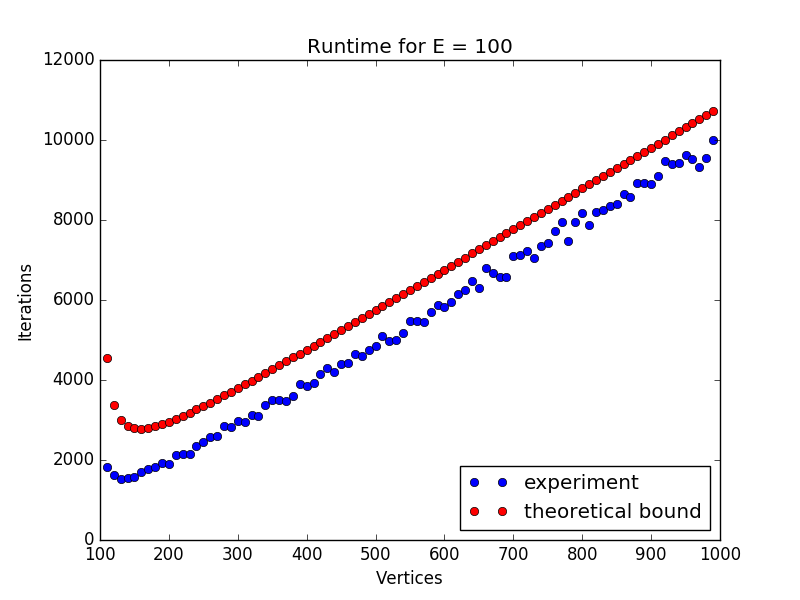
\includegraphics[width=10cm]{pic/rarefied_graph.png}
 \end{frame}


\end{document}